\section{完全四边形}
\subsection{密克尔点}
\begin{definition}[密克尔(Miquel)点]
    设在$\triangle ABC$的每条边所在直线上取一点,过三角形的每一顶点与两条邻边上所取的点作圆,则这三个圆交于一点,该点通常称作密克尔点。
\end{definition}
\begin{figure}[htbp]
    \centering
    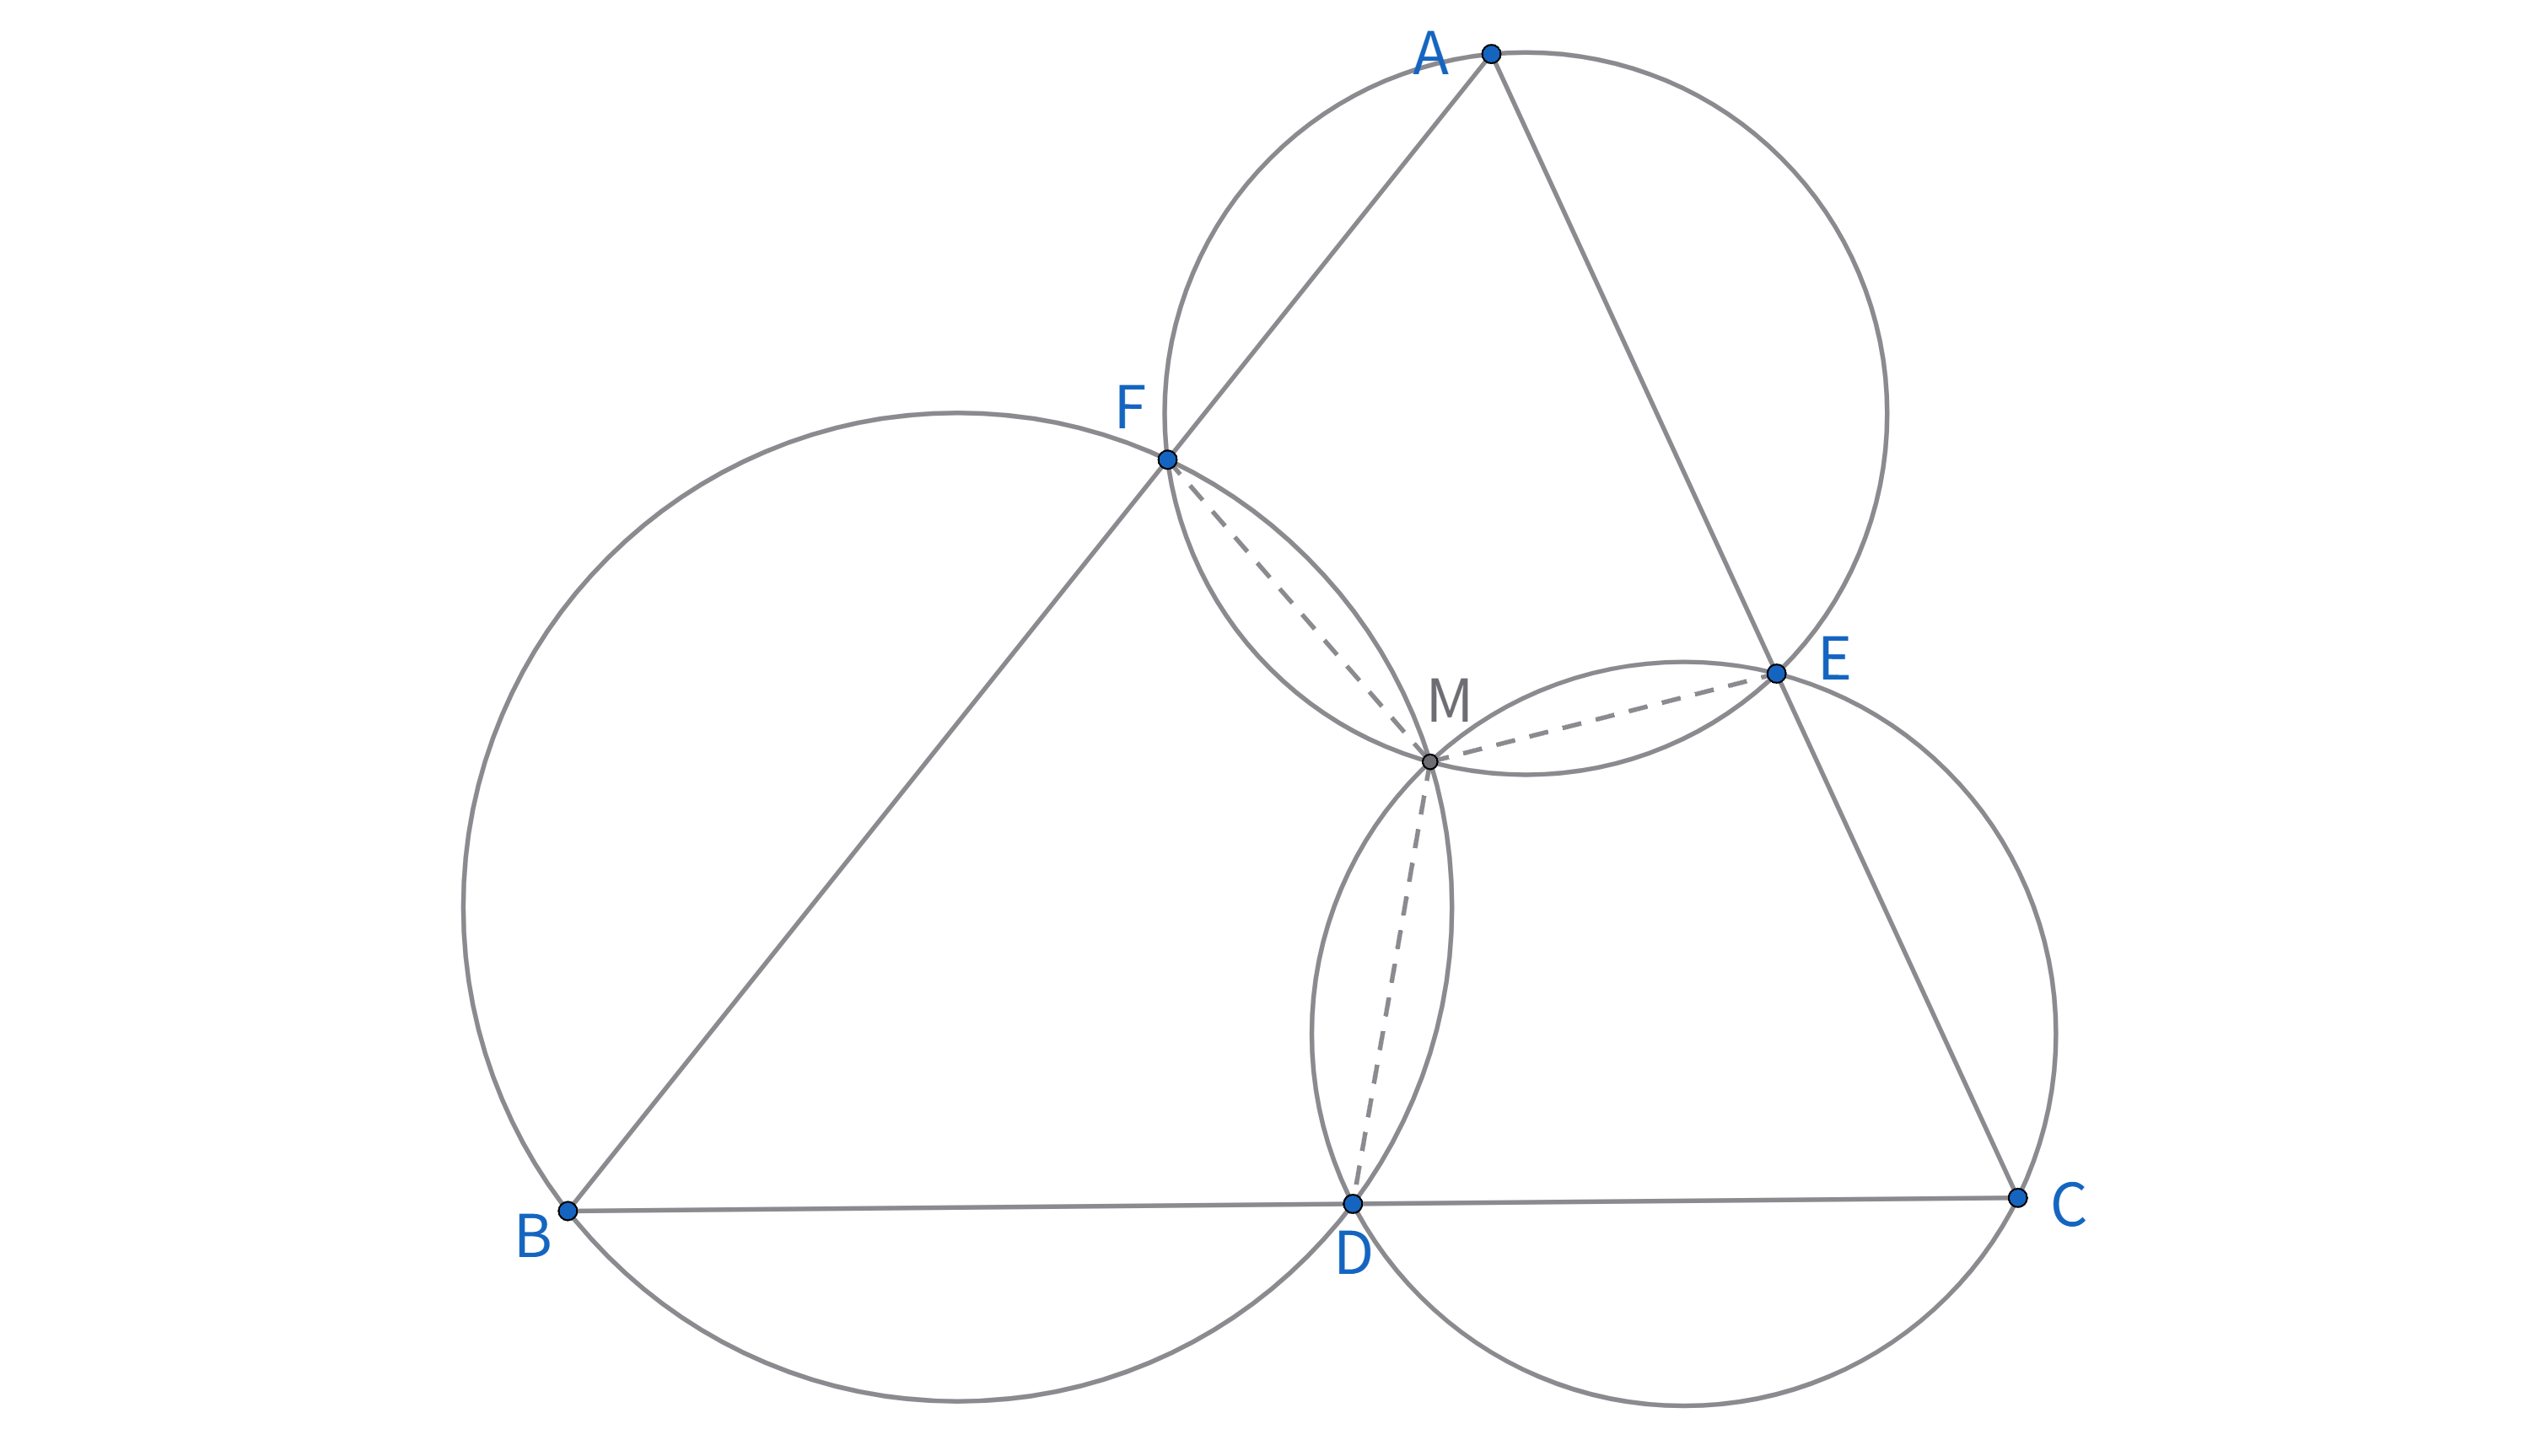
\includegraphics[width=\linewidth]{figures/密克尔点.png}
    \caption{密克尔点}
\end{figure}


\newpage 
\subsection{完全四边形}
\begin{definition}
    两两相交又没有三线共点的四条直线以及它们的六个交点所构成的图形,称作完全四边形。
    六个点可分成三对相对的顶点,它们的连线是三条对角线。
\end{definition}
\begin{figure}
    \centering
    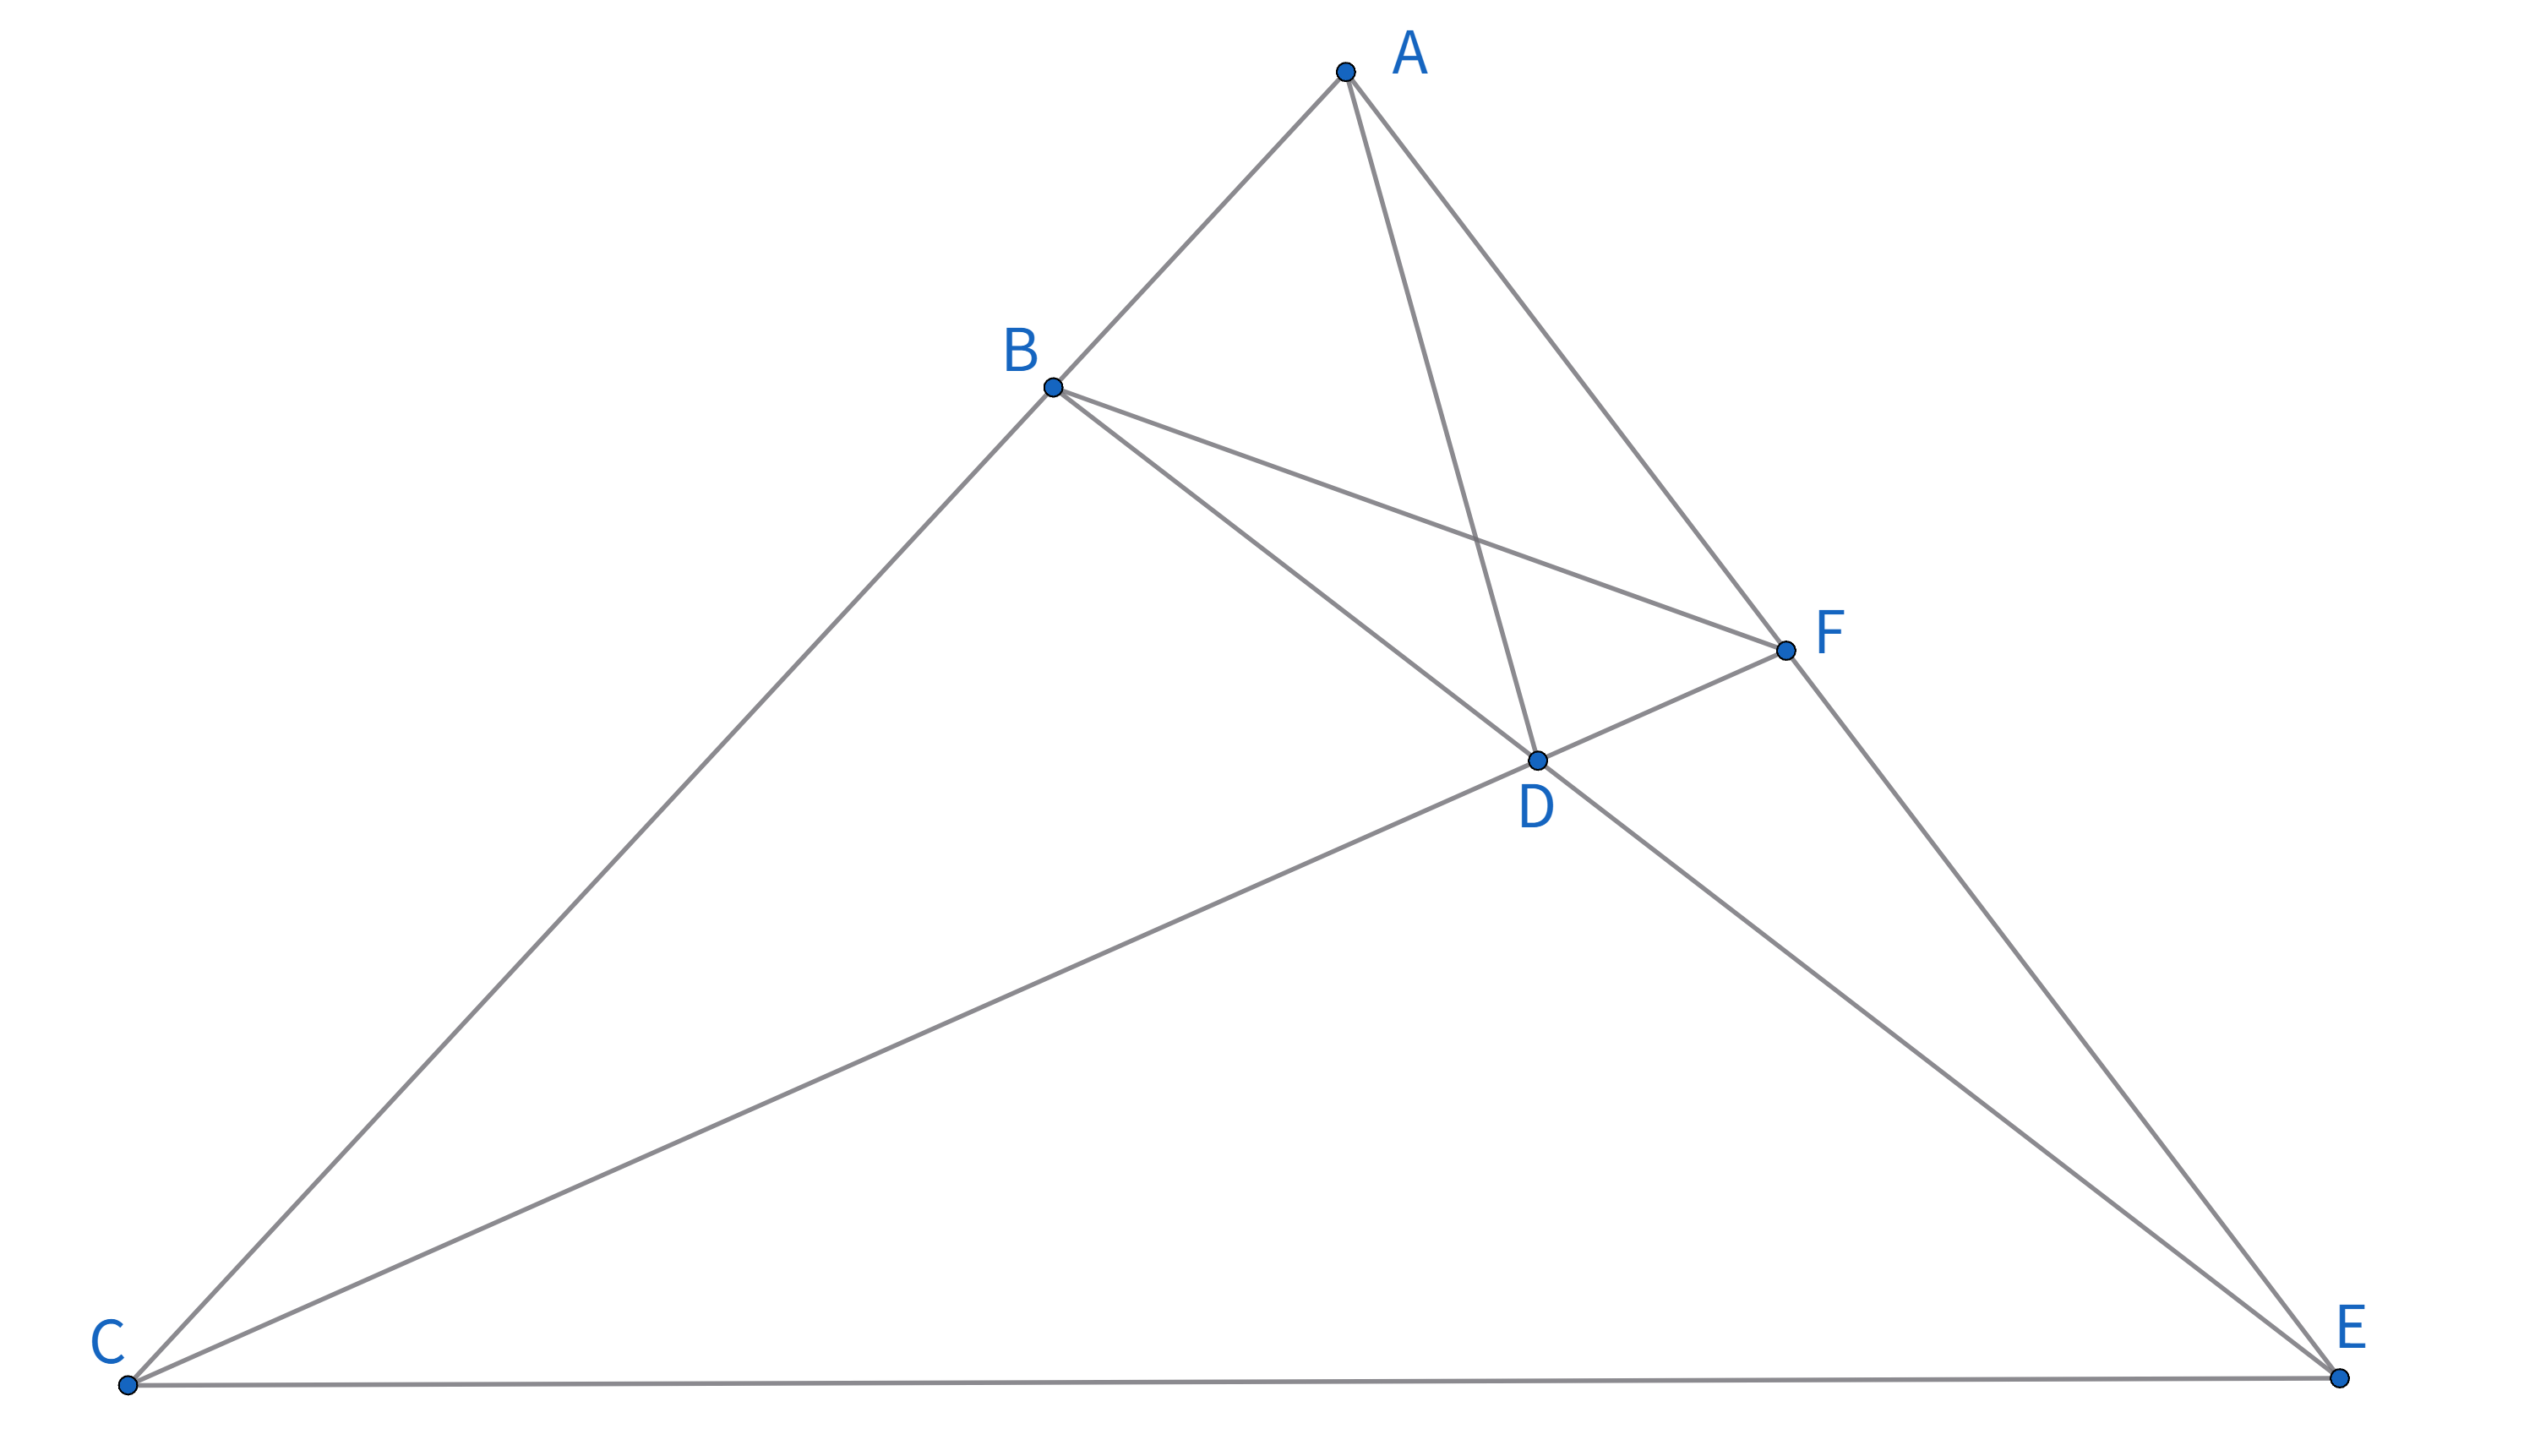
\includegraphics[width=0.5\linewidth]{figures/完全四边形.png}
    \caption{完全四边形}
\end{figure}

\newpage 
\begin{theorem}[完全四边形的密克尔点]
    四条一般位置的直线形成的四个三角形,它们的外接圆共点。
\end{theorem}
\begin{figure}[htbp]
    \centering
    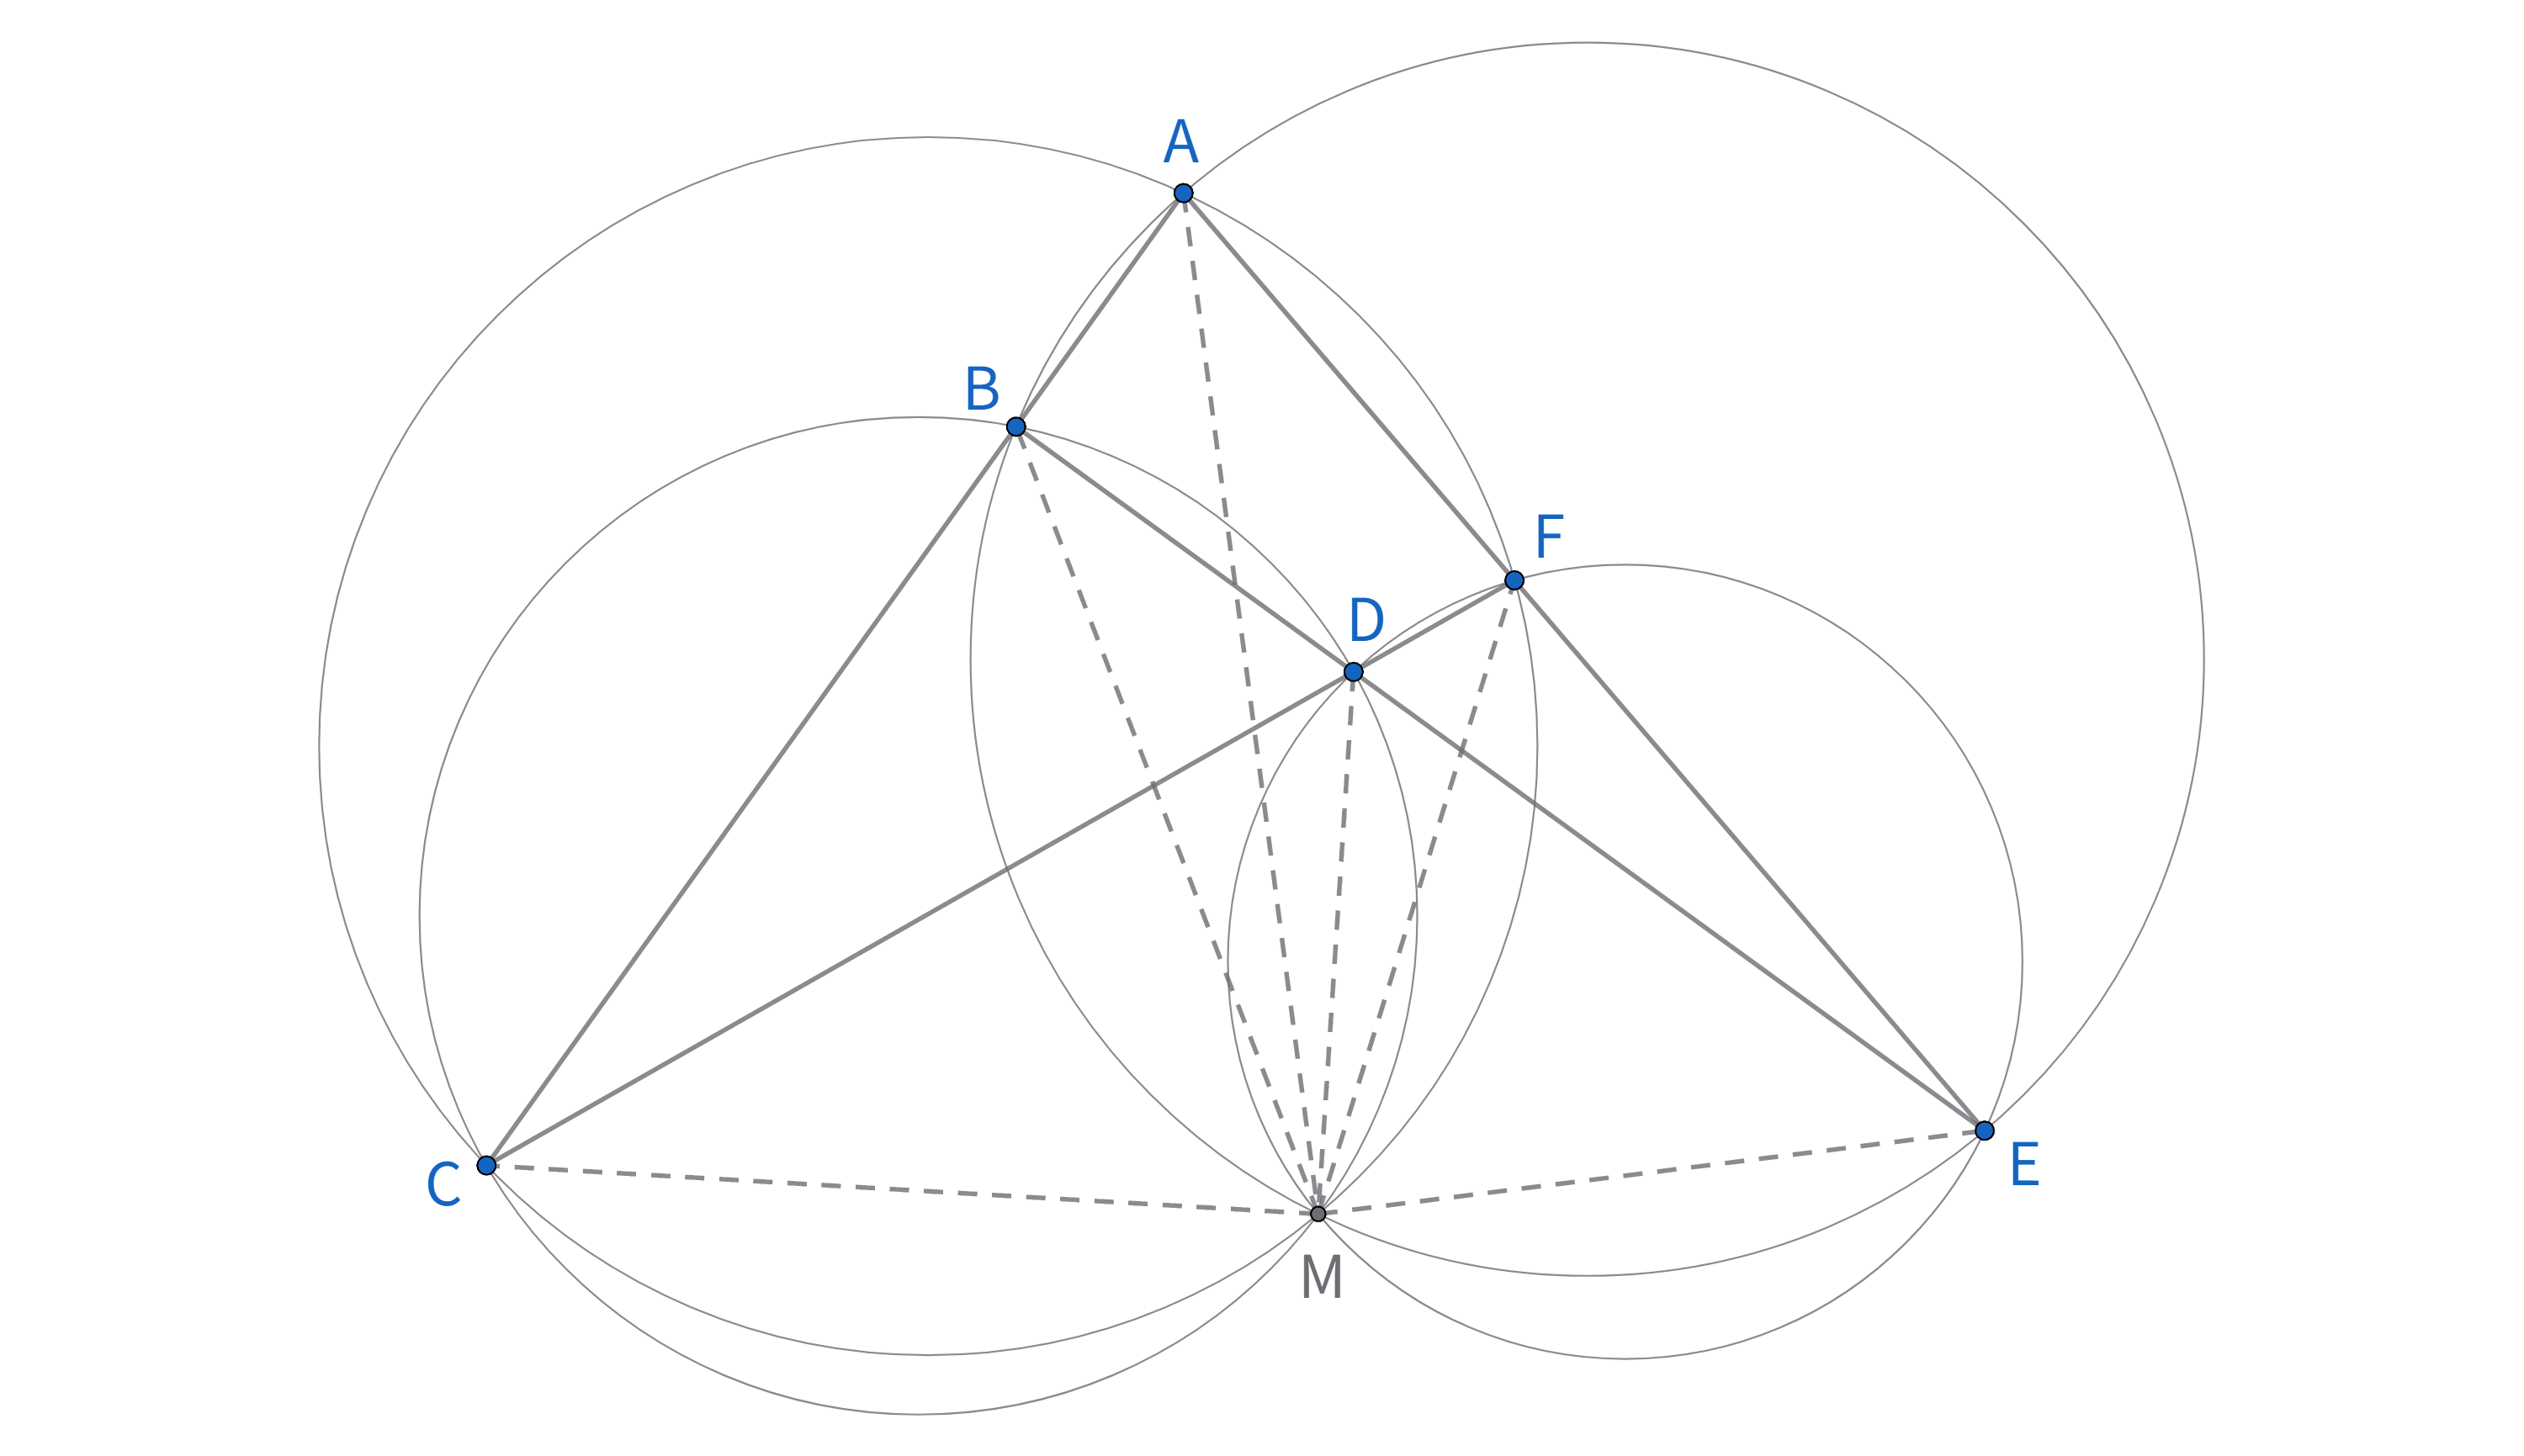
\includegraphics[width=\linewidth]{figures/完全四边形密克尔点.png}
    \caption{完全四边形的密克尔点}
\end{figure}

\newpage
\begin{proposition}
    
\end{proposition}